\section{Referencial Teórico}
\label{sec:referencialTeorico}
% Os principais conceitos aos quais os trabalho está relacionado. Por exemplo, apresentar os conceitos de Aprendizado de Máquina e métodos relacionados.
% As principais técnicas e métodos nos quais o trabalho se apoia (referências)

Antes de tratar sobre as definições mais específicas que este trabalho vai utilizar, gostaria de trazer uma definição mais geral em que o problema está incluído. Podemos compreender Sistemas de Informação como sistemas, sejam eles manuais ou automatizados, inter-relacionados que atuam armazenando, processando e transmitindo dados que representam informações para as partes interessadas (\textit{stakeholders}). De forma mais geral, esses sistemas \enquote{\textit{atuam em conjunto para o cumprimento de uma tarefa ou um objetivo}} \cite{turban2009business}.

O grupo básico de operações de um Sistema de Informação é constituído pelas entradas, pelo processamento e pelas saídas (Figura \ref{fig:operacoesBasicaSistemas}). A entrada é o conjunto de dados que será usado pelo sistema, o processamento é composto pela transformações e combinações que os dados de entradas serão submetidos e, por fim, a saída é o produto obtido por meio do processamento dos dados de entrada. Em alguns casos, o sistema pode ser retroalimentado (\textit{feedback}), fazendo com que o resultado de saída seja manipulado como dados de entrada em uma nova execução. Nesse processo, também é comum que ocorra o armazenamento dos dados de entrada e de saída para serem utilizados posteriormente, como pode ser visto na Figura \ref{fig:operacoesBasicaSistemas}.

\begin{figure}[ht]
\centering
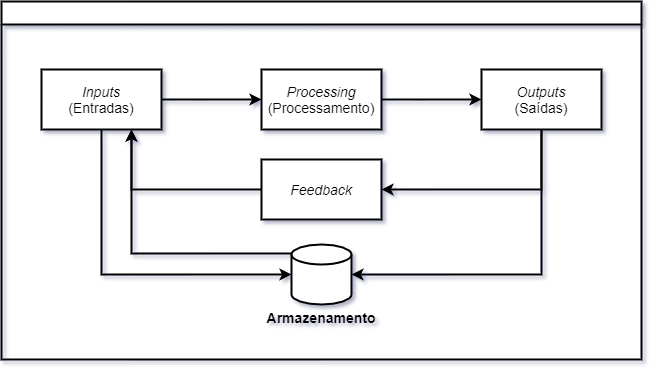
\includegraphics[width=1\textwidth]{imagens/operacoes-basicas-sistema-informacao.png}
\caption{Operações básicas de um Sistema de Informação.}
\label{fig:operacoesBasicaSistemas}
\end{figure}

Os dados que servem como entrada do sistema \enquote{\textit{são a menor parte de uma informação}}, \cite{boscarioli2016mineracao}, e podem ser definidos como conhecimento bruto ou fatos isolados. Nesse estado, podemos tê-los como não adequadamente tratados para fornecer gnose aos \textit{stakeholders}.

Por sua vez, a informação é a saída do sistema e descreve \enquote{\textit{qualquer conhecimento do mundo real... mas que apresenta algum significado ou valor para quem o detém}} \cite{boscarioli2016mineracao}. A informação é formada pelos dados de entrada do sistema após serem transformados, combinados \enquote{\textit{relacionados logicamente e organizados para atingir um resultado definido}}, \cite{vida2021datawarehouse}, passando a fornecer conhecimento relevante para o processo de tomada de decisão.

Dessa maneira, temos os dados como matéria-prima do sistema e a informação como o produto. O nome de uma pessoa, uma data e um valor monetário são bons exemplos de dados, isolados eles não significam muito. No entanto, quando combinamos esses dados e atribuímos um significado ou contexto, como um depósito bancário, eles, os dados, passam a ter valor e se tornam informação.

Depois do processamento dos dados, e também antes, como já foi dito, os dados que compõem/comporão a informação precisam ser armazenados de maneira organizada. Para realizar essa organização é comum usar um banco de dados relacional (Figura \ref{fig:bancoDadosRelacional}), no qual \enquote{\textit{são conjuntos de dados organizados e relacionados entre si com registros sobre fatos, pessoas, empresas, coisas ou lugares.}} \cite{rezende2015obi}. Em vista disso, os bancos de dados são essenciais para os sistemas de informação.

\begin{figure}[ht]
\centering
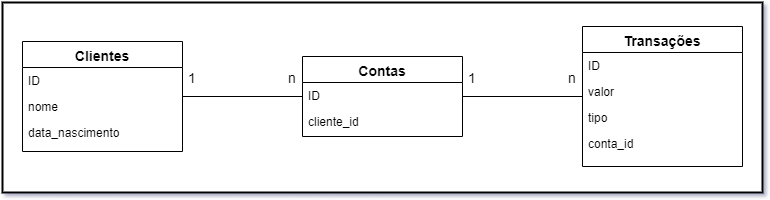
\includegraphics[width=1\textwidth]{imagens/banco-relacional.png}
\caption{Exemplo de descrição das tabelas de um banco de dados relacional}
\label{fig:bancoDadosRelacional}
\end{figure}

Vale destacar que um conjunto de dados composto por dados aleatórios não pode ser qualificado como um banco de dados, pois existem algumas características que devem ser atendidas para que seja classificado como tal.

\begin{itemize}
  \item \textbf{Minimundo}: O banco de dados deve representar uma parte do mundo real \cite{vida2021datawarehouse}.
  \item \textbf{Dados com significado}: O banco de dados também tem que ser constituído por um conjunto lógico de dados que apresente algum significado \cite{vida2021datawarehouse}.
  \item \textbf{Dados com objetivo}: Os dados que integram o banco necessitam ter ou cumprir um objetivo claro para o usuário ou aplicação, sendo prescindível o armazenamento dos dados que não contribuem com o propósito \cite{vida2021datawarehouse}.
\end{itemize} 

% \hfill

\subsection{Data Warehouse}
\label{subsec:datawarehouse}

Ao longo das décadas, os computadores tiveram a sua capacidade de processamento e armazenamento aumentadas e juntamente com eles, houve um aumento da necessidade das empresas de investigar um grande volume de dados para nortear a sua tomada de decisão. Diante dessa necessidade, muitas abordagens foram criadas e \enquote{\textit{em 1988, o braço irlandês da IBM lançou o termo business data warehouse para valorizar os dados empresarias que estavam sendo armazenados. Em 1990, surgiu uma abordagem que ficou conhecida como data warehouses, sendo responsável pela cópia dos dados armazenados em arquivos e em banco de dados para outro local.}} \cite{vida2021datawarehouse}.

Os dados que ficam armazenados nesse \enquote{novo} banco de dados (\textit{data warehouse}) são provindos de diversas base de dados oriunda das distintas áreas da empresa. Com isso, os \textit{data warehouses} foram concebidos para consolidar o conhecimento dessa pluralidade de base de dados. De maneira simplória, podemos dizer que os \textit{data warehouses} são nada mais que imensos banco de dados ou, como o nome sugere, armazém de dados que mantêm muitas informações históricas que, normalmente, não serão apagadas. Ainda podemos considerar os \textit{data warehouses} como um conjunto ampliável e organizado de dados arquitetado com a finalidade de analisar dados historiais, relevantes para o negócio, de diversas fontes. Um \textit{data warehouse} também deve manter a consistência dos dados, garantindo que não sejam modificados ou corrompidos. Os passos para a crianção de um \textit{data warehouse} podem ser descritos por \enquote{\textit{coleta, consolidação, análise e pesquisa}}, \cite{vida2021datawarehouse}.

Dentre as vantagens do uso de \textit{data warehouses} estão a diminuição da redundância de informações, já que ele centraliza os dados de diversas fonte e elimina as cópias desnecessárias. A padronização é outra vantagem, pois facilita a sua manipulação e análise, além de manter a integralidade da informação e torna a consulta mais acessível.

Existem quatro termos que apresentam características importantíssimas do \textit{data warehouse}: \enquote{\textit{orientado por assuntos, integrado, variável no tempo e não volatilidade}}, \cite{vida2021datawarehouse}.

Um \textit{data warehouse} orientado por assuntos contém dados importantes e concernente ao negócio, ou seja, a organização das informações estão voltadas para o \enquote{assunto}, diferente dos bancos de dados convencionais que são orientados a processos ou funções. Dessa maneira, um \textit{data warehouse} não deve armazenar dados que não são \enquote{realmente} necessários para o negócio.

Todos os dados do \textit{data warehouse} estão integrados, isso quer dizer que nele não existem dados não integrados, em nenhum caso \cite{turban2009business}. Para ser consistente é necessária a padronização dos dados que entram no \textit{data warehouse}, tornando-os simples e universais. As práticas mais comuns que introduzem inconsistências no banco são \enquote{\textit{Codificação e Forma dos atributos}}, \cite{vida2021datawarehouse}. A codificação ocorre quando uma informação pode ser expressada de diversas maneiras. Um exemplo disso é um dado boleando que pode ser expresso por \enquote{verdadeiro} e \enquote{falso}, \enquote{0} e \enquote{1}, \enquote{sim} e \enquote{não}, etc. Já a forma dos atributos pode introduzir inconsistência quando são utilizadas medidas diferentes como graus celsius e kelvin, metro e milha, grama e onça.

A variável de tempo é essencial em cada registro de um \textit{data warehouse}. Isso é indispensável para se ter um sistema histórico de dados. Esse sistema pode ser apresentado de maneira simples, como uma linha do tempo, ou mais complexa e detalhada. \enquote{\textit{Os dados em um data warehouse podem ser considerados uma longa série de snapshots}}, \cite{boscarioli2016mineracao}, ou seja, semelhante a uma coleção de registros de vários momento no tempo (diário, semanal, mensal, anual, etc.) e análogo a documentos que não podem ser alterados (apesar de ocorrer em momentos excepcionais, mesmo sendo incorreto).

A não volatilidade do \textit{data warehouse} diz respeito as operações feitas nele. Enquanto um banco de dados comum tem por operações ordinárias a seleção, inclusão, atualização e exclusão, o \textit{data warehouse} executa somente a carga inicial e a consulta dos dados, isto significa que o dados não são alterados ou excluídos dentro dele o que o torna, nesse aspecto, mais simples que um banco de dado comum.

Existem duas abordagens quanto ao modelo de um \textit{data warehouse}, a abordagem relacional e a abordagem multidimensional. Na abordagem relacional os dados são organizados em um formato de tabela de duas dimensões (linhas e colunas). Nessa perspectiva, cada registro é uma linha da tabela, que por sua vez é dividida em colunas. Já o modelo multidimensional arranja as tabelas de um banco de dados relacional de modo a expressar os dados em várias dimensões por meio de tabelas de fatos e tabelas de dimensão usando esquemas em estrela (Figura \ref{fig:esquemaEstrela}) ou em floco de neve (Figura \ref{fig:esquemaFlocoNeve}). O esquema em estrela usa uma tabela de fato central que é ligada a várias tabelas de dimensão, nas quais cada tabela desse tipo representa uma dimensão. Enquanto isso, o esquema em floco de neve é uma extensão do esquema em estrela, pois ele possui a mesma organização em fatos e dimensões, porém, adicionando tabelas de \enquote{subdimensão} relacionadas às tabelas de dimensão. Enquanto as tabelas do esquema em estrela não são normalizadas, isto é, podem ter dados repetidos, as tabelas do esquema em floco de neve são normalizadas graças as tabelas adicionais, o que reduz a redundância.

% Fonte da imagem https://www.educba.com/star-schema-vs-snowflake-schema/
\begin{figure}[ht]
\centering
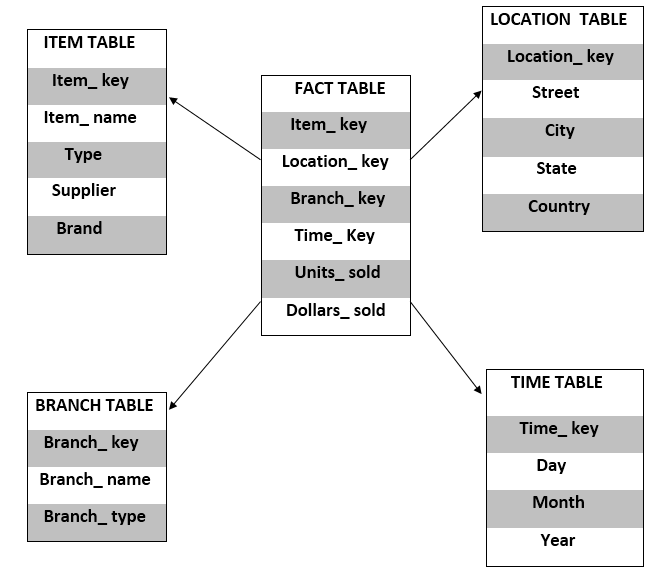
\includegraphics[width=.8\textwidth]{imagens/example-star-schema.png}
\caption{Esquema em estrela.}
\author{Fonte: https://www.educba.com/star-schema-vs-snowflake-schema/}
\label{fig:esquemaEstrela}
\end{figure}

% Fonte da imagem https://www.educba.com/star-schema-vs-snowflake-schema/
\begin{figure}[ht]
\centering
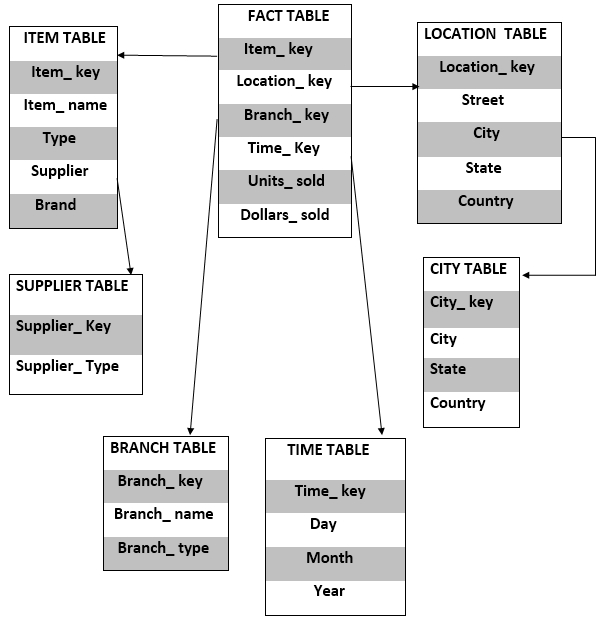
\includegraphics[width=.8\textwidth]{imagens/example-snowflake-schema.jpg}
\caption{Esquema em floco de neve}
\author{Fonte: https://www.educba.com/star-schema-vs-snowflake-schema/}
\label{fig:esquemaFlocoNeve}
\end{figure}

\subsection{ETL}
\label{subsec:etl}
O \textit{data warehouse} é uma ótima maneira de armazenar grandes quantidades de dados provenientes de diversas fontes. Essa enorme massa de dados é agrupada com o objetivo de criar um ambiente preparado para efetuar análises complexas para auxiliar na tomada de decisão por meio da descoberta de informações sobre os diferentes setores do seu negócio.

A fim de que um \textit{data warehouse} se mantenha atualizado para fornecer boas inspirações, é necessário que ele seja carregado de tempos em tempos (diária ou semanalmente, por exemplo, sempre observando o impacto que a carga causa aos sistemas de origem e também atentando à necessidade de atualização dos dados), transcrevendo os dados das variadas fontes de origem para dentro dele. Esse processo de copiar os dados das fontes, transformá-los para se ajustar ao esquema do \textit{data warehouse} e carregá-los no próprio \textit{data warehouse} é conhecido por ETL (Figura \ref{fig:processoETL}), sigla em inglês para \textit{Extract, Transform and Load} ou extração, transformação e carga, em uma tradução livre. Desse modo, os dados importantes das fontes são enriquecidos para gerar informações úteis que serão depositadas no \textit{data warehouse}.

As principais etapas do ETL são definidas da seguinte forma:

\begin{itemize}
  \item \textbf{Extração}: Consiste no processo de ler os dados de uma fonte de dados particular e extrair dele um subconjunto de dados \cite{goarETL}.
  \item \textbf{Transformação}: Corresponde ao método de modificação/combinação dos dados extraídos previamente para adequá-los aos requisitos da nova base de dados \cite{goarETL}.
  \item \textbf{Carga}: O processo de escrever os dados transformados anteriormente no base de dados objetivo (\textit{data warehouse}) \cite{goarETL}.
\end{itemize} 

\begin{figure}[ht]
\centering
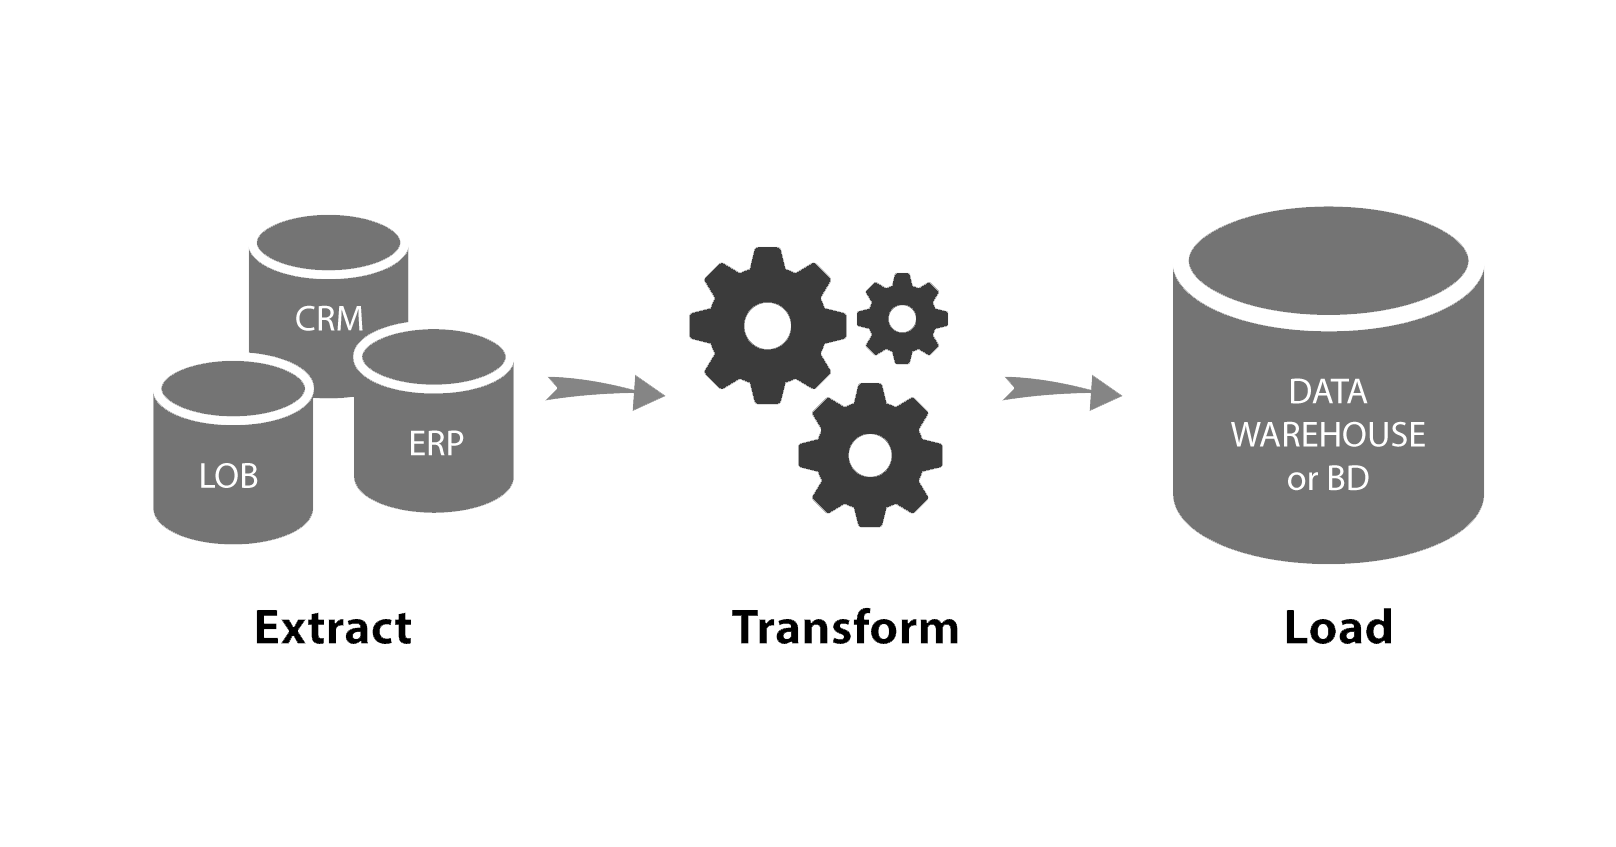
\includegraphics[width=1\textwidth]{imagens/etl-processo.png}
\caption{Representação do processo de ETL}
\author{Fonte: https://blog.indicium.tech/etl-vs-elt-diferencas/}
\label{fig:processoETL}
\end{figure}

Essa tarefa de carga do \textit{data warehouse} pode ser bastante complexa, pois os dados que são oriundos das diversas bases de dados podem seguir padrões distintos uns dos outros. Por isso, se faz necessária a extração, limpeza e formatação, transformação e integração apropriada para não prejudicar a qualidade das consultas realizadas no \textit{data warehouse}. De acordo com especialistas do setor, aproximadamente 60-80 porcento do esforço empregado em um projeto de \textit{data warehouse} é aplicado no processo de ETL \cite{goarETL}.

\subsubsection{Extração}
\label{subsec:extracao}
A extração é a primeira etapa do ETL, nela os dados serão extraídos das mais diversas fontes, bancos de dados, sistemas de arquivos, páginas da \textit{web}, etc, para uma área intermediária conhecida como \textit{staging area} ou área de preparação. Essa transferência de dados é feita para reduzir a carga sobre os sistemas que detêm as fontes de dados e também do próprio \textit{data warehouse}. Nesse ponto, os dados, sejam eles estruturados ou não estruturados, são importados em uma organização estável e de fácil consulta para um único local. Na área de preparação serão feita as transformações necessárias para adequar os dados aos requisitos do destino, o \textit{data warehouse}, por isso, ainda não é possível criar qualquer tipo de relatório para o usuário final ou  realizar consulta neste sentido.

\subsubsection{Transformação}
\label{subsec:transformacao}
A partir da área de preparação, segue-se com a etapa de transformação dos dados. Essa etapa é responsável por modificar os dados brutos e estruturá-los para que estejam adequados para serem introduzidos no \textit{data warehouse} de destino. As transformações aplicadas aqui seguem as regras de negócio já estabelecidas para enriquecer os dados, aumentando a sua qualidade. Essas conversões também têm o objetivo de tornar os dados mais acessíveis e fazer com que os relatórios gerados no \textit{data warehouse} atendam os requisitos do negócio.

Existem diversos tipos de atividades de transformação de dados que são realizadas nessa etapa. Abaixo estão listadas algumas da mais comuns:

\begin{itemize}
  \item Limpeza, filtragem, eliminação de informações duplicadas, validação e autenticação de dados \cite{vida2021datawarehouse}.
  \item Execução de cálculos, traduções ou resumos dos dados brutos, conversões de moedas ou unidades de medida, padronização da codificação das \textit{strings} \cite{vida2021datawarehouse}.
  \item Ocultação de dados sensíveis ou protegidos por regulamentações governamentais ou de setores específicos da empresa \cite{vida2021datawarehouse}.
  \item Estruturar os dados em forma de tabelas para condizer com o esquema do \textit{data warehouse} final \cite{vida2021datawarehouse}.
  \item \enquote{\textit{Outras tarefas com o objetivo de melhorar a qualidade dos dados.}}, \cite{vida2021datawarehouse}.
\end{itemize} 

A etapa de transformação é a parte mais custosa, computacionalmente, do ETL, devido a isso, é recomendado que ela seja executada na área de preparação para não afetar negativamente o desempenho da própria etapa, dos sistemas que originam os dados e do \textit{data warehouse}.

% TODO começar a falar de ETL - Carga
\subsubsection{Carga}
\label{subsec:carga}
Por fim, temos a etapa de carga. Ela é a responsável por transferir os dados após serem transformados, copiando-os da área de preparação para o \textit{data warehouse} de destino para serem usados na geração de visões que guiarão a tomada de decisão. A carga pode ser realizada de dua maneiras, a carga total ou a carga incremental, que ocorre em períodos programados.

O carregamento total é quando \enquote{\textit{tudo o que vem da linha de montagem de transformação}}, \cite{vida2021datawarehouse}, vai para o \textit{data warehouse}. Ela é bastante útil quando se quer realizar pesquisas, no entanto, os dados podem crescer desmedidamente, o que tornar esse processo muito custoso. É comum que esse tipo de carga ocorra fora do horário comercial, de maneira automatizada, para evitar sobrecarregar o \textit{data warehouse} enquanto ele é usado pelos usuários finais.

Já o carregamento incremental introduz os dados no \textit{data warehouse} frequentemente, em cargas programadas. No entanto, é feito um carregamento inicial com todos os dados, para, somente após isso, os dados serem inseridos regularmente. Nesse método, os dados só serão incluídos caso não existam registros idênticos no sistema objetivo, escrevendo somente as informações novas e ignorando linhas de lançamentos antigos. Esse tipo de abordagem permite a construção de \textit{data warehouses} menos custosos por baratear a sua manutenção, além de permitir que novos dados sejam incluídos rapidamente no \textit{data warehouse}, viabilizando uma tomada de decisão mais veloz. Contudo, é comum que sejam feitas caragas completas no \textit{data warehouse} para substituir todos os dados contidos nele, mas isso ocorre em uma frequência menor.

O ETL de um \textit{data warehouse} pode ser organizado em forma de \textit{pipeline}, no qual as etapas são conectadas em série de modo que a saída de um passo sirva como entrada do passo posterior. Dessa forma, os estágios do ETL podem ser executados em paralelo, permitindo que vários registros sejam processados simultaneamente, eliminando a necessidade de esperar que um registro passe por todo o ETL para então iniciar o processamento próximo registro \cite{vida2021datawarehouse}.

% TODO Inserir imagem da página 167 do livro.  "Pipeline das funções ETL"

Assim, o ETL é projetado para fornecer valor ao negócio da empresa por meio da união dos dados, do enriquecimento, da estruturação, da padronização e da eliminação de redundância que eles podem conter. Ele também eleva a qualidade dos dados e permite que os \textit{stakeholders} possam acessar e manipular as informações oriundas de diversas fontes com facilidade e clareza. Outro ponto positivo é que o ETL aumenta o campo de visão da análise, devido à integralidade dos dados proveniente do máximo de fontes relevantes reunidas em um único local, no caso, o \textit{data warehouse}. À vista disso, podemos dizer que o processo de ELT amplia os horizontes da empresa tanto pela qualidade e completude das informações que são entregues, permitindo que as decisões tomadas sejam apoiadas em dados reais, quanto pelo tempo que ele dá aos \textit{stakeholders} por retirar deles o trabalho de reunir essa grande quantidade de dados.